%!TEX root = ../main.tex
% TODO schema model checker
% TODO riferimenti articoli ctl pctl
% TODO riferimento a javapathfinder
% TODO sintassi e semantiche in tabelle

\myChapter{Model Checking}
Garantire l'assenza di errori in sistemi complessi come i software è un problema di grande interesse sia nell'ambiente dell'industria che in quello della ricerca. Nel primo settore si sono diffusi svariati strumenti tra cui il \emph{testing}, le \emph{simulazioni} e le \emph{peer review} al fine di far fronte al problema. Il testing è una tecnica dinamica che spesso si appoggia a componenti di terzi e ad attività di \emph{mock-up}, cioè anteprime parziali a scopo esplicativo dei requisiti richiesti. Si sono diffuse anche tecniche di sviluppo orientate al testing: partendo dai requisiti si ricercano i test che il sistema (ancora inesistente) dovrà superare, quindi si passa allo sviluppo supervisionato da verifiche costanti. Il principale problema del testing è che fornisce una copertura solamente parziale di quello che viene richiesto e in sistemi complessi come ad esempio i \emph{software multithread} gli interleaving che si creano sono un numero impossibile da gestire. Anche per le simulazioni valgono gli stessi punti elencati per il testing: possono garantire che il caso simulato sia corretto ma non che l'intero sistema lo sia.

La tecnica di peer review consiste nello scambio di codice tra programmatori. Anche in questo caso però diventa impossibile gestire sistemi concorrenti per l'elevato numero di interleaving.

Il \emph{model checking} è un metodo formale che affronta il problema della correttezza di un sistema. La tecnica si basa sulla costruzione di un modello astratto che rappresenti il sistema e di una formula che rappresenti il requisito da soddisfare. Entrambi gli elementi devono essere espressi in modo formale secondo una struttura nota per poter rendere questo metodo automatizzabile. Il \emph{model checker} (figura \ref{fig:modelchecker}) è quindi uno strumento che prende in ingresso la rappresentazione del sistema e la formula e risponde con un esito positivo se il sistema la soddisfa, negativo altrimenti, possibilmente fornendo un controesempio.
\begin{figure}[htb]
	\begin{center}
		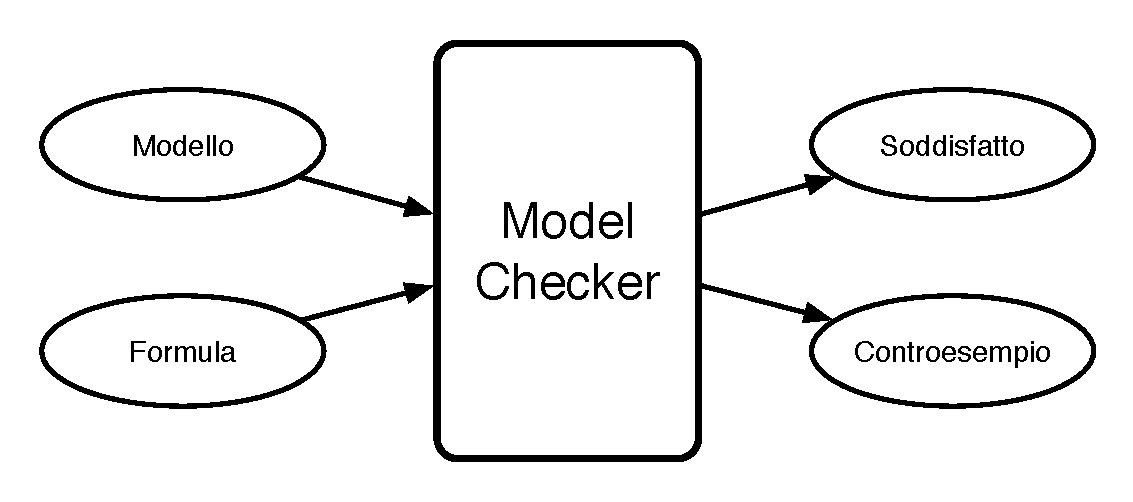
\includegraphics[width=.8\textwidth]{Images/mc.eps}
	\end{center}
\caption{Schema del funzionamento di un model checker}
\label{fig:modelchecker}
\end{figure}

In un contesto reale è spesso impossibile pensare di ottenere un sistema complesso totalmente privo di errori o imperfezioni, si rilassano quindi le richieste introducendo dei gradi di tolleranza degli errori. Un caso concreto può essere il gestore di una compagnia telefonica che permette di effettuare un'alta percentuale di chiamate senza problemi di interferenze o interruzioni, ad esempio il $98\%$. Oltre al modello e alla formula viene quindi introdotto nel model checker il parametro dell'\emph{accuratezza} che rende una formula verificata se il grado di fallimento rientra nella tolleranza espressa. Un model checker a cui si aggiunge un parametro di accuratezza espresso in probabilità viene chiamato \emph{probabilistic model checker} (figura \ref{fig:probabilisticmodelchecker}).
\begin{figure}[htb]
	\begin{center}
		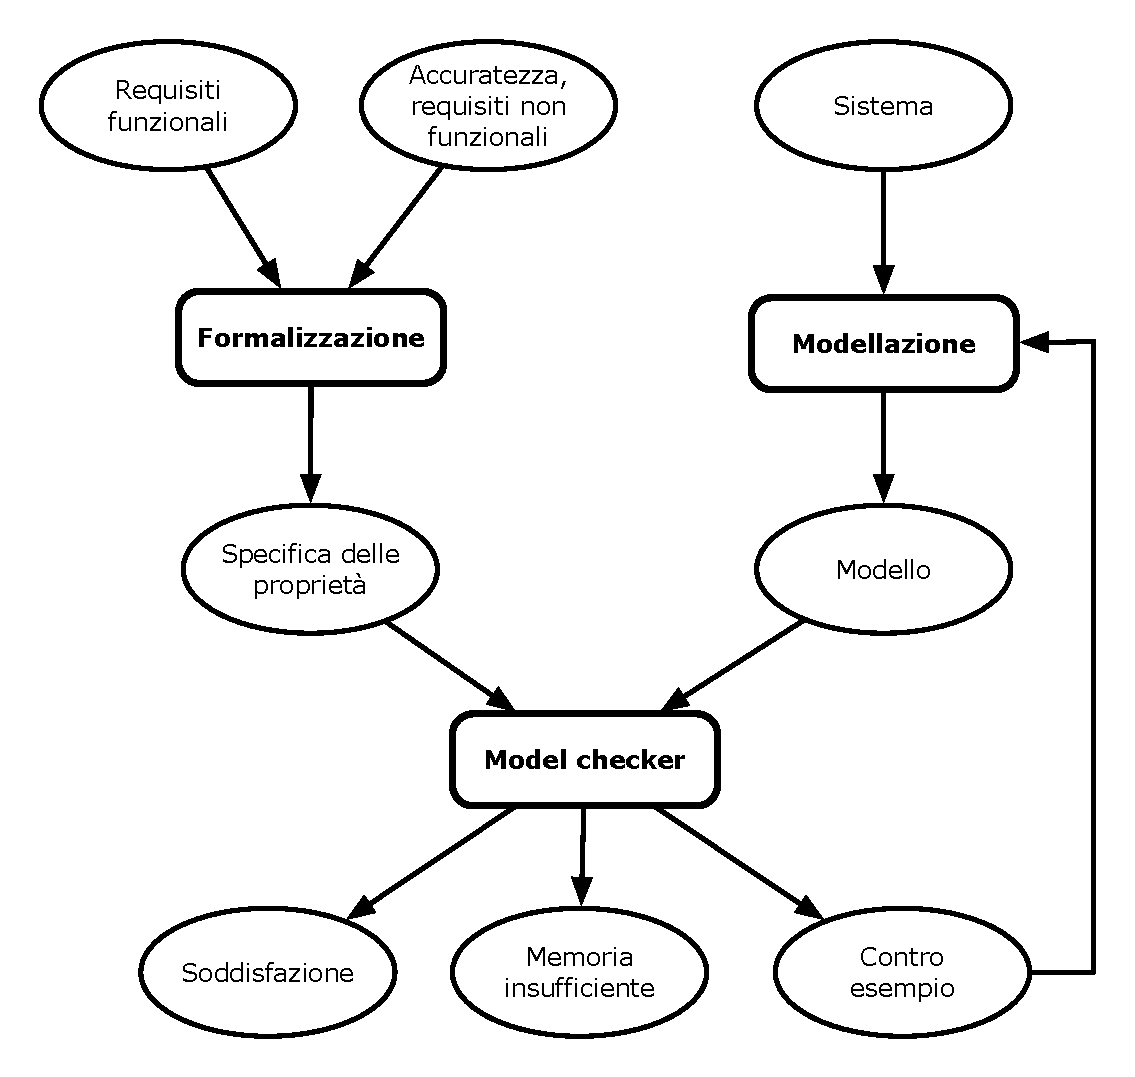
\includegraphics[width=\textwidth]{Images/pmc.eps}
	\end{center}
\caption{Schema del funzionamento di un model checker probabilistico}
\label{fig:probabilisticmodelchecker}
\end{figure}

Dalla formalizzazione dei requisiti si può ottenere un insieme di proprietà che dovranno essere soddisfatte. Più precisamente, dai requisiti \emph{funzionali} possiamo ottenere le formule di proprietà da soddisfare, mentre quelli \emph{non funzionali} forniscono l'accuratezza da utilizzare. Dopo aver fornito al model checker il modello del sistema, la proprietà da verificare e l'accuratezza, questo può produrre tre tipi di risposte:
\begin{itemize}
	\item la proprietà viene soddisfatta dal modello nei limiti richiesti,
	\item la memoria non è sufficiente per portare a termine la verifica oppure
	\item la proprietà non viene soddisfatta dal modello, fornendo un controesempio.
\end{itemize}
Se non si riceve esito positivo si può intervenire a seconda di che tipo di problema è stato riscontrato. Nel secondo caso si verifica il fenomeno conosciuto come \emph{esplosione degli stati} che ha origine quando si vuole modellare sistemi molto complessi, come i già citati software multithread. La conseguenza è una richiesta di memoria e tempo di calcolo proibitivi. Per far fronte a questo problema si ricorre spesso alla scomposizione del sistema in sotto sistemi e ad astrazioni di modelli troppo complessi. Ovviamente se invece non viene soddisfatta la formula è necessario intervenire sul modello stesso cercando di correggere i comportamenti erronei evidenziati.

Il model checking viene utilizzato in modo diverso se ci troviamo prima o dopo la fase di sviluppo: nel primo caso è necessario costruire il modello astratto del sistema, nel secondo, invece, è possibile utilizzare degli strumenti (i.e. \emph{java path finder}) per effettuare le verifiche direttamente sul codice. 

\section{Probabilit\`a elementari}
Introduciamo le misure principali utilizzate dei model checker probabilistici, assumendo di utilizzare come strutture dei modelli le \ac{dtmc} e le \ac{mdp}. Esistono due tipi di misure di probabilità elementari delle \ac{dtmc}:
\begin{itemize}
	\item probabilità \emph{transiente} e
	\item probabilità \emph{a regime}, o \emph{steady state}.
\end{itemize}

\begin{mtdef}[Probabilità transiente $\pi_j(n)$]
La probabilità \emph{transiente} $\pi_j(n) = \mathbb{P}\{X_n = j\}$ è la probabilità che la \ac{dtmc} sia nello stato $j$ al passo $n$
\end{mtdef}

Possiamo quindi associare alla \ac{dtmc} $\mathcal{D}$ un vettore che al passo $n$ descriva la probabilità di trovarsi in ogni stato $s \in S$ $$\underline\pi(n) \triangleq (\pi_1(n), \dots, \pi_{|S|}(n)).$$
Si indica con $\underline\pi(0)$ la distribuzione di probabilità iniziale mentre con $\underline\pi(n)$ la distribuzione di probabilità al passo $n$.
Considerando che moltiplicare il vettore di distribuzione di probabilità per la matrice $\mathbb{P}$ rappresenta un avanzamento del sistema che aggiorna la distribuzione al passo successivo, allora vale la seguente \emph{relazione di ricorrenza}
$$ \underline\pi(n) = \underline\pi(n-1) \cdot \mathbb{P} $$
da cui si ricava immediatamente la seguente forma dipendente solo dalla  distribuzione iniziale e dalla matrice di transizione
$$ \underline\pi(n) = \underline\pi(0) \cdot \mathbb{P}^n$$

\begin{mtdef}[Probabilità steady state $\pi_j$]
La probabilità \emph{steady state} $$\pi_j = \lim_{n\rightarrow\infty} \mathbb{P}\{X_n = j\}$$ è la probabilità che la \ac{dtmc} sia a regime nello stato $j$.
\end{mtdef}

L'esistenza di questo limite è garantita solo sotto determinate condizioni di \emph{ergodicità} della catena. Supponendo che il limite sia indipendente dalla distribuzione iniziale, per calcolare questa distribuzione è sufficiente risolvere il seguente sistema di equazioni lineari
$$
\left\{
\begin{array}{l}
\underline\pi \cdot \mathbb{P} = \underline\pi \\
\sum^{|S|}_{i=1} \pi_i = 1 \\
\end{array}
\right.
$$
dove $0 \leq \pi_i \leq 1$ e $1 \leq i \leq |S|$.

Una volta scelto uno scheduler che risolva le scelte nondeterministiche della \ac{mdp} trasformandola in una \ac{dtmc} sarà possibile applicare la valutazione delle probabilità sopra descritte. Il risultato però sarà valido solo in presenza di quello specifico scheduler che potrebbe avere un peso poco rilevante nell'analisi della \ac{mdp}. Quello che si fa quindi è calcolare il range di probabilità in cui si muove la misura interessata \emph{per ogni} possibile scheduler in modo da poter fare inferenza su \emph{lower} e \emph{upper bounds}.

\section{Probabilistic Computation Tree Logic}
Al fine di poter effettuare model checking su strutture come \ac{dtmc} e \ac{mdp} utilizziamo \ac{pctl}, un'estensione probabilistica della logica temporale \ac{ctl}. Il linguaggio \ac{pctl} è uno strumento che permette di esprimere specifiche di interesse sulla struttura che stiamo condiderando. Può essere quindi utilizzato sia sulle \ac{dtmc} che sulle \ac{mdp} adattando la struttura alla potenza espressiva del modello. In generale le formule che esprimono specifiche in modo formale hanno un ruolo fondamentale all'interno del model checking in quanto permettono di rendere automatico il procedimento di verifica.

In seguito riportiamo la sintassi e la semantica di \ac{pctl} definita per le \ac{mdp}, più generale rispetto a quella per le \ac{dtmc} ed effettivamente impiegata all'interno di questo lavoro.

\begin{mtdef}[Sintassi \ac{pctl}]
	La sintassi \ac{pctl} viene definita come segue:
$$
\begin{array}{rcl}
	\phi &::=& true \Sep \mathit{a} \Sep \phi_1 \wedge \phi_2 \Sep \neg\phi \Sep \mathcal{P}_{\bowtie p}[\psi] \\
	\psi &::=& \mathcal{X}\phi \Sep \phi_1 \mathcal{U}^{\leq k} \phi_2 \Sep \phi_1 \mathcal{U} \phi_2 \\
\end{array}
$$
dove $\mathit{a}$ è una proposizione atomica, $\bowtie \in \{\leq,<,\geq,>\}$, $p \in[0,1]$ e $k \in \mathbb{N}$.
\end{mtdef}
Dalla sintassi distinguiamo due tipi di formula: le formule di stato $\phi$ e le formule di cammino $\psi$. Per definire formalmente la semantica è necessario specificare come gli elementi dell'insieme $AP$ delle proposizioni atomiche sono gestiti in una \ac{mdp}.
\begin{mtdef}[\ac{mdp} etichettata]
	Una \ac{mdp} etichettata è una tupla $(\mathcal{M},L)$ dove:
	\begin{itemize}
		\item $\mathcal{M}$ è una \ac{mdp};
		\item $L:S\rightarrow 2^{AP}$ è una funzione di etichettatura.
	\end{itemize}
\end{mtdef}
Estendiamo quindi la struttura delle \ac{mdp} con una funzione $L$ che associa ad ogni stato un certo insieme di proposizioni atomiche. A questo punto abbiamo tutti gli strumenti per definire la semantica di \ac{pctl} secondo una relazione di soddisfacibilità.
\begin{mtdef}[Relazione di soddisfacibilità]
	Sia $\mathcal{M} = (S,\overline{s},Act,Steps,L)$ una \ac{mdp} etichettata. Per ogni stato $s \in S$, la relazione di soddisfacibilità di stato $\models$ è definita per induzione come segue:
$$
	\begin{array}{rllcl}
		\mathcal{M},s &\models& \phi &\Leftrightarrow& \mathcal{M},s \models_{st} \phi \\
		\mathcal{M},s &\models_{st}& true && \forall s \in S, \\
		\mathcal{M},s &\models_{st}& \mathit{a} &\Leftrightarrow& \mathit{a} \in L(s), \\
		\mathcal{M},s &\models_{st}& \neg\phi &\Leftrightarrow& s \not\models_{st} \phi, \\
		\mathcal{M},s &\models_{st}& \phi_1 \wedge \phi_2 &\Leftrightarrow& s\models_{st}\phi_1 \ e\ s\models_{st}\phi_2, \\
		\mathcal{M},s &\models_{st}& \mathbb{P}\{ \mathcal{P}_{\bowtie p}[\psi]\} &\Leftrightarrow& p_s^\Sigma(\psi)\bowtie p,\ \forall\ \Sigma \in Scheduler_\mathcal{M}, \\
	\end{array}
$$
dove per ogni scheduler $\Sigma \in Scheduler_\mathcal{M}$:
$$
p_s^\Sigma \triangleq Prob_s^\Sigma(\{\pi \in Path_s^\Sigma \sep \pi \models_{pt} \psi\})
$$
e per ogni cammino $\pi \in Path$:
$$
\begin{array}{rclcl}
	\mathcal{M},\pi & \models_{pt} & \mathcal{X}\phi & \Leftrightarrow & \mathcal{M},\pi(1) \models_{pt} \phi, \\
	\mathcal{M},\pi & \models_{pt} & \phi_1 \mathcal{U}^{\leq k} \phi_2 & \Leftrightarrow & \exists i \leq k\ .\ (\mathcal{M},\pi(i) \models_{pt} \phi_2\ e\ \mathcal{M},\pi(j) \models_{pt} \phi_1 \forall j < i), \\
	\mathcal{M},\pi & \models_{pt} & \phi_1 \mathcal{U} \phi_2 & \Leftrightarrow & \exists k \geq 0\ .\ \mathcal{M},\pi \models_{pt} \phi_1 \mathcal{U}^{\leq k} \phi_2. \\
\end{array}
$$
\end{mtdef}

Per specificare una formula \ac{pctl} si utilizza sempre una formula di stato che al suo interno potrà utilizzare formule di cammino. Intuitivamente gli operatori logici possono essere utilizzati per indagare sulle proposizioni atomiche contenute in un determinato stato, mentre l'operatore $\mathcal{P}_{\bowtie p}[\psi]$ viene soddisfatto dagli stati che soddisfano la formula di cammino $\psi$ con una probabilità nell'intervallo specificato da $\bowtie p$. Questo operatore si comporta sempre nel modo appena descritto se i cammini non incontrano scelte nondeterministiche (nelle \ac{dtmc} è sempre vero) ma come deve comportarsi in caso contrario? Dato che non si può assumere niente sulle suddette scelte e sfruttando il fatto che l'applicazione di uno scheduler ad una \ac{mdp} produce una \ac{dtmc}, l'operatore è considerato soddisfatto se la condizione è valida \emph{per qualsiasi scheduler}.

Per quanto riguarda le formule di cammino, l'operatore \emph{next} $\mathcal{X}\phi$ richiede che $\phi$ venga soddisfatta dallo stato successivo, l'operatore \emph{bounded until} $\phi_1 \mathcal{U}^{\leq k} \phi_2$ richiede che $\phi_2$ venga soddisfatto entro $k$ passi e che $\phi_1$ resti sempre soddisfatto fino a quel punto, mentre l'operatore \emph{unbonded until} $\phi_1 \mathcal{U} \phi_2$ richiede che prima o poi $\phi_2$ venga soddisfatto e che $\phi_1$ sia sempre soddisfatto fino a quel punto.

Possiamo rielaborare i construtti principali definiti finora per estendere il linguaggio con degli operatori derivati (tabella \ref{tab:sintassi:derivati}). Mentre gli operatori logici $false$, $\vee$ e $\rightarrow$ possono essere derivati facilmente, vi sono alcuni operatori meno banali. Gli operatori $\Diamond$ e $\Box$ sono molto comuni nelle logiche temporali e servono a specificare rispettivamente proprietà che hanno speranza di avverarsi in futuro e proprietà che sicuramente non si verificheranno mai. Delle applicazioni interessanti di questi due concetti sono le proprietà di \emph{liveness} e di \emph{safety}. Una proprietà di \emph{liveness} esprime la possibilità che prima o poi accada qualcosa di positivo mentre la duale \emph{safety} indica che qualcosa di negativo non potrà mai accadere. I due operatori possono essere usati per descrivere queste due tipologie proprietà ma sono più generali. 
Le varianti \emph{bounded} $\Diamond^{\leq k}$ e $\Box^{\leq k}$ stabiliscono, tramite il numero di passi $k \in \mathbb{N}$, il tempo entro il quale la proprietà $\phi$ deve rimanere soddisfatta a partire dall'istante iniziale. La proprietà di cammino $\Diamond^{\leq k}\phi$ sarà quindi soddisfatta se entro $k$ passi $\phi$ si verificherà almeno una volta, mentre la proprietà di cammino $\Box^{\leq k}$ sarà soddisfatta se $\phi$ rimarrà sempre soddisfatta per tutti e $k$ i passi. 
Per definire gli operatori $\Box$ e $\Box^{\leq k}$ viene introdotta la notazione $\overline\bowtie$ che rappresenta l'inversione degli operatori secondo le seguenti equivalenze: $\overline\leq \equiv \geq$, $\overline < \equiv >$, $\overline\geq \equiv \leq$ e $\overline > \equiv <$.
Un ultimo operatore interessante è il quantificatore esistenziale $\exists$ che \emph{ricerca l'esistenza di uno scheduler} che soddisfa una certa formula, contrariamente all'approccio generale basato sulla soddisfacibilità di tutti i possibili scheduler.
\begin{table}[htbp!]
$$
\begin{array}{rcl}
	false & \equiv & \neg true \\
	\phi_1 \vee \phi_2 & \equiv & \neg(\neg\phi_1 \wedge \neg\phi_2) \\
	\phi_1 \rightarrow \phi_2 & \equiv & \neg\phi_1 \vee \phi_2 \\
	\mathcal{P}_{\bowtie p}[\Diamond \phi] & \equiv & \mathcal{P}_{\bowtie p}[true \mathcal{U} \phi] \\
	\mathcal{P}_{\bowtie p}[\Diamond^{\leq k} \phi] & \equiv & \mathcal{P}_{\bowtie p}[true \mathcal{U}^{\leq k} \phi] \\
	\mathcal{P}_{\bowtie p}[\Box \phi] & \equiv & \mathcal{P}_{\overline\bowtie 1-p}[\Diamond \neg \phi] \\
	\mathcal{P}_{\bowtie p}[\Box^{\leq k} \phi] & \equiv & \mathcal{P}_{\overline\bowtie 1-p}[\Diamond^{\leq k} \neg \phi] \\
	\exists\Diamond\phi & \equiv & \neg \mathcal{P}_{\leq 0}[\Diamond\phi] \\
\end{array}
$$
\caption{Operatori derivati di \acs{pctl}}
\label{tab:sintassi:derivati}
\end{table}

\section{PRISM model checker}
Il model checker probabilistico che utilizzeremo è \prism{} \cite{KNP11}. Si tratta di un tool con il quale è possibile fare modellazione e analisi di sistemi che presentano aspetti probabilistici. I principali modelli probabilistici supportati sono le \ac{dtmc}, le \ac{mdp}, le \ac{ctmc} ed i \ac{pta}, mentre i linguaggi utilizzabili per descrivere le formule sono \ac{pctl}, \ac{csl} e \ac{ltl}. In questa sezione descriveremo l'utilizzo di \prism{} concentrandoci sugli strumenti di interesse diretto per questo lavoro come le \ac{mdp} e il linguaggio \ac{pctl} precedentemente descritti.

\prism{} utilizza un suo specifico linguaggio con il quale è possibile definire tutti i modelli sopra citati. Si tratta infatti di un linguaggio basato sugli stati e su formalismi tipici dei sistemi reattivi. I componenti fondamentali rappresentati dal linguaggio sono i \emph{moduli} e le \emph{variabili}, un \emph{modello} viene rappresentato come un insieme di moduli che possono interagire tra loro. Ogni modulo può inoltre contenere delle variabili locali e il valore di queste variabili ad un certo istante rappresentano il suo stato. Allo stesso modo lo stato del modello globale è definito come lo stato locale di tutti i moduli che lo compongono.

Il comportamento di un modulo viene definito dall'insieme di \emph{comandi} che contiene. Un comando ha la seguente forma:
\begin{verbatim}
	[] guardia -> prob_1 : update_1 + ... + prob_n : update_n ;
\end{verbatim}
La \emph{guardia} è un predicato che può considerare qualsiasi variabile del modello e se risulta soddisfatta il modello può avanzare eseguendo una delle transizioni \emph{update} con le rispettive probabilità (o evenutalmente rate). L'intero modulo viene definito specificandone il nome e il contenuto
\begin{verbatim}
	module name ... endmodule
\end{verbatim}
All'interno del modulo possono essere presenti sia comandi che variabili. Al fine di avere uno \emph{spazio finito di stati} \prism{} permette di gestire solo variabili booleane e variabili intere in un range finito. Di seguito mostriamo la dichiarazione di una variabile $x$ che può assumere i valori interi compresi tra $0$ e $10$ compresi inizializzata a 5 e una variabile booleana $b$ inizializzata a $true$:
\begin{verbatim}
	x : [0..10] init 5;
	b : bool init true;
\end{verbatim}
Le guardie sono classiche espressioni booleane che possono fare riferimento a variabili di qualsiasi modulo in quanto viene richiesta solamente la lettura dei valori. Gli update, invece, sono sequenze di assegnamenti intervallate dal separatore $\&$. La sequenza di update vuota viene indicata con $true$. Un assegnamento di un valore a una variabile può avvenire solo su una variabile locale al modulo a cui appartiene il comando, inoltre il nome della variabile aggiornata deve terminare col simbolo $'$ ad indicarne il nuovo stato. All'interno del listato \ref{code:prism:example1} mostriamo l'utilizzo degli strumenti appena descritti. L'esempio rappresenta due processi in mutua esclusione.
\begin{lstlisting}[language=prism,style=eclipse,caption={Esempio di definizione dei moduli in \prism{}},label=code:prism:example1]
module M1

x : [0..2] init 0;

    [] x=0 -> 0.8:(x'=0) + 0.2:(x'=1);
    [] x=1 & y!=2 -> (x'=2);
    [] x=2 -> 0.5:(x'=2) + 0.5:(x'=0);

endmodule 

module M2

y : [0..2] init 0;

    [] y=0 -> 0.8:(y'=0) + 0.2:(y'=1);
    [] y=1 & x!=2 -> (y'=2);
    [] y=2 -> 0.5:(y'=2) + 0.5:(y'=0);

endmodule
\end{lstlisting}
In questo caso i due moduli sono simmetrici, ed entrambi presentano esclusivamente scelte probabilistiche. Possiamo se necessario inserire anche delle scelte non deterministiche sulle quali è quindi impossibile fare osservazioni di tipo quantitativo. Modificando il modulo $M1$ come mostrato nel listato \ref{code:prism:example2} inseriamo una scelta nondeterministica, infatti le due nuove guardie insierite saranno sempre abilitate insieme.
\begin{lstlisting}[language=prism,style=eclipse,caption={Scelta nondeterministica in \prism{}},label=code:prism:example2]
module M1

x : [0..2] init 0;

	// scelta nondeterministica
    [] x=0 -> (x'=0);
	[] x=0 -> (x'=1);
	
    [] x=1 & y!=2 -> (x'=2);
    [] x=2 -> 0.5:(x'=2) + 0.5:(x'=0);
	
endmodule
\end{lstlisting}
In generale il nondeterminismo può verificarsi anche se due guardie vengono soddisfatte assieme anche solo parzialmente. La stessa struttura può quindi presentare scelte deterministiche a seconda dello stato corrente.

In \prism{} è anche possibile definire delle costanti globali sui domini di interi, reali e booleani:
\begin{verbatim}
	const int z = 12;
	const double pi = 3.141592;
	const bool flag = true;
\end{verbatim}
Queste costanti possono essere utilizzate, al fine di parametrizzare il modello, all'interno delle espressioni che possono coinvolgere i seguenti operatori:
\begin{itemize}
	\item $-$ meno unario, $*$ moltiplicazione, $\slash$ divisione, $+$ somma e $-$ sottrazione,
	\item le relazioni d'ordine $<$, $\leq$, $>$, $\geq$, e di equivalenza $=$ e $!=$
	\item gli operatori booleani di $!$ negazione, $\&$ congiunzione, $|$ disgiunzione, $<=>$ se e solo se e $=>$ implicazione logica.
\end{itemize}
Sono presenti inoltre le funzioni:
\begin{itemize}
	\item $min$ minimo e $max$ massimo,
	\item $floor$ di arrotondamento all'intero minore più vicino,
	\item $ceil$ di arrotondamento all'intero maggiore più vicino,
	\item $pow$ per l'elevamento a potenza,
	\item $mod$ modulo,
	\item $log$ logaritmo.
\end{itemize}
Le espressioni possono essere utilizzate non solo nelle condizioni delle guardie, nelle inizializzazioni e negli aggiornamenti, ma anche per calcolare le proprietà di una transizione.

Come primo parametro di un comando può essere inserita la label di un'azione per far sincronizzare i moduli. Un azione viene quindi specificata inserendone il nome (ad esempio \emph{step}) all'interno delle parentesi quadre, nel seguente modo
\begin{verbatim}
	[step] x=0 -> 0.8:(x'=0) + 0.2:(x'=1);
\end{verbatim}

Il modello finale viene ricavato di default dalla \emph{composizione parallela} di tutti i moduli che lo compongono, se si vuole invece descrivere una composizione diversa, è possibile usare il costrutto
\begin{verbatim}
	system ... endsystem
\end{verbatim}
Al suo interno possono essere usati i seguenti operatori \ac{csp}:
\begin{itemize}
	\item $M1\ ||\ M2$: i moduli si sincronizzano solo su azioni che appaiono in entrambi (composizione parallela di default),
	\item $M1\ |||\ M2$: interleaving completo, senza sincronizzazione,
	\item $M1\ |[a,b,...]|\ M2$: la sincronizzazione avviene solo sulle azioni specificate nell'operatore,
	\item $M \slash \{a,b,...\}$ le azioni specificate vengono nascoste all'esterno,
	\item $M \{a<-b,c<-d,...\}$ le azioni vengono rinominate all'esterno.
\end{itemize}
Alcuni esempi di espressioni di sistema sono mostrati di seguito:
\begin{verbatim}
	system (station1 ||| station2 ||| station3) |[serve]| server endsystem
	system ((P1 |[a]| P2) / {a}) || Q endsystem
	system ((P1 |[a]| P2) {a<-b}) |[b]| Q endsystem
\end{verbatim}
